\documentclass[12pt]{report} % Type du document
\usepackage[french]{babel} % Langue du document
\usepackage[T1]{fontenc}
\usepackage[utf8]{inputenc}
\usepackage[left=15mm, right=15mm]{geometry} % Définition de la largeur des marges gauches et droites

\usepackage{a4wide} % Format de la feuille
\usepackage{amsmath} % Pour inclure des équations
\usepackage{graphicx} % Pour inclure des images / graphiques
\usepackage{float} % Pour gérer le placement des images
\usepackage{fancyhdr} % Pour les headers, paramètres ci-dessous
\usepackage{listings} %Pour afficher du code formaté
\usepackage{subcaption}

\graphicspath{ {images/} }

% Paramètres fancyhdr
\pagestyle{fancy}
\rhead{Basile Botebol, Baptiste Hardrick}
\lhead{
\includegraphics[width=1.5cm]{HEIG.png}}
\cfoot{\thepage} % thepage affiche le numéro de page courant
\setlength{\parindent}{0cm}

\title{\textbf{SOS 2019\\Securité Des OS\\Laboratoire 1 - Windows}} % '\\' force un retour à la ligne (Bonne pratique: Réserver ça aux titres)
\author{Basile Botebol, Baptiste Hardrick}
\date{Mai 2019} % Laisser vide pour ne pas afficher la date 


\begin{document}

\maketitle

\section*{Reconnaissance}

\subsection*{Réponses aux questions}
\par P1: -Pn traite tous les hôtes comme étant en ligne -> cela permet de passer outre la découverte des hôtes

\par P2: WAD-DC-SRV2\\
On peut le déterminer en faisant les manipulations présentées dans le laboratoire (en scannant le port 445 (smb)) 
et en regardant leur nom (celui dont le nom comporte DC)\\
La deuxième méthode se fait en scannant grâce à un nmap sur port 88 car c'est sur ce port que tourne kerberos qui est 
propre au domain controler.


\subsection*{Résultat des Manipulations}

\begin{figure}[!h]
	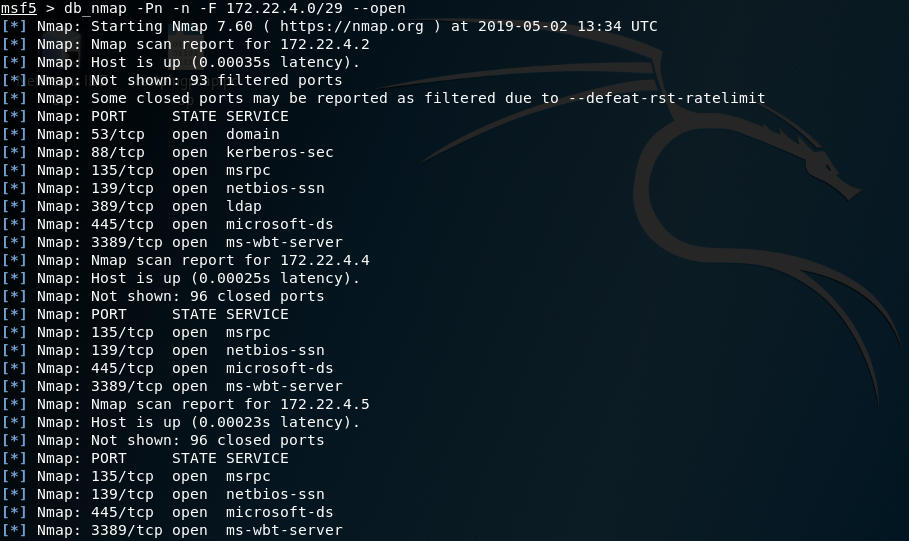
\includegraphics[width=17cm, height=13cm]{db_nmap_3_1_a.PNG}
	\caption*{Résultat du db nmap - partie 1}
\end{figure}

\begin{figure}
	\newpage
	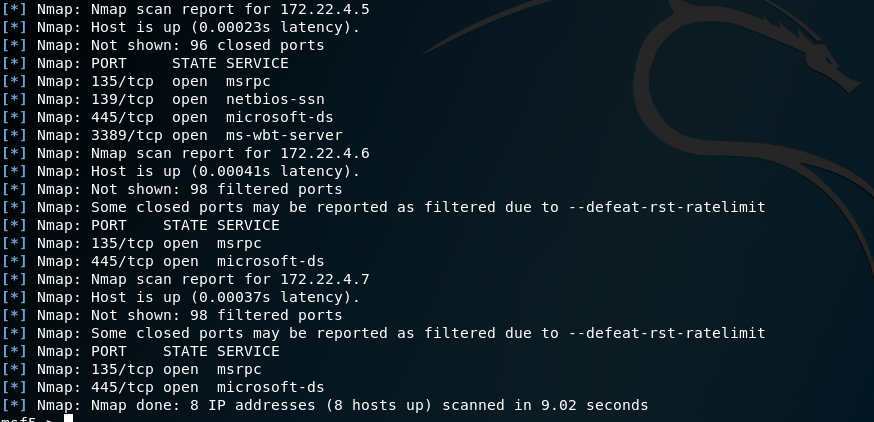
\includegraphics[width=17cm, height=13cm]{db_nmap_3_1_b.PNG}
	\caption*{Résultat du db nmap - partie 2}
\end{figure}

\newpage

\section*{Exploitation de vulnérabilités logicielles}

\subsection*{Réponses aux questions}
\par P3: ip vulnérable: On obtient les droits d'exécution SYSTEM
\par P4: La faille MS17-010 permet à l'attaquant d'exécuter n'importe quelle commande et donc, d'avoir les privilèges system.
\par P5: 188 powershell.exe (grâce aux commandes getpid et ps dans le meterpreter)
\par P6: Un reverse shell fait en sorte que la victime vienne se connecter à un port définit par l'attaquant (sur sa machine) alors qu'un bind shell consiste à ouvrir un port sur la machine de la victime et à s'y connecter.
\par P7: Il est recommandé d'utiliser un reverse shell lorsqu'il y a un firewall protegeant la victime (qui risquerait d'empecher un bind)
\par P8: Il s'agit de composants payload (comme Meterpreter dans notre cas) qui sont téléchargés depuis un Stager.
Les Stagers permettant eux de créer une connection entre l'attaquant et la victime.

\newpage
\subsection*{Résultat des Manipulations}
\begin{figure}[!h]
	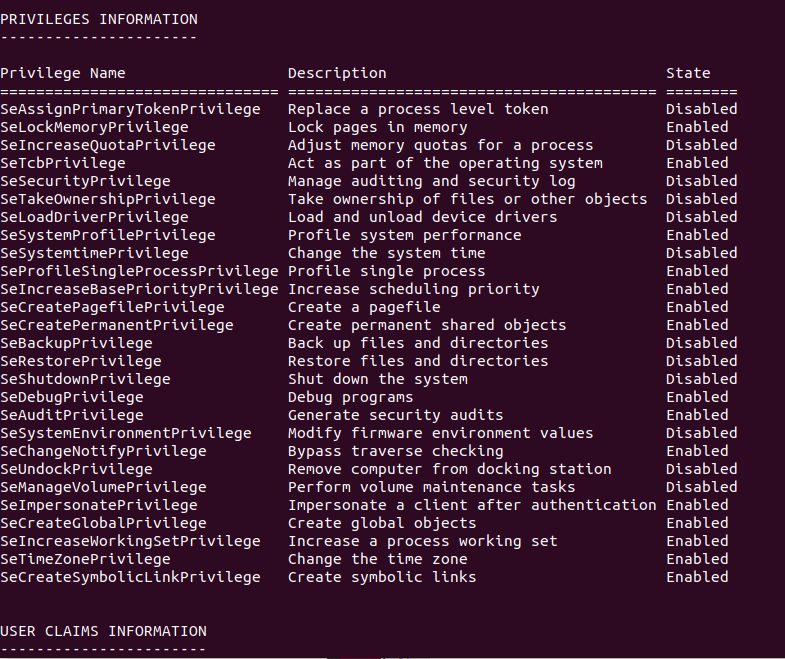
\includegraphics[width=17cm, height=13cm]{Privileges_3_2.PNG}
	\caption*{Liste des privilèges obtenus}
\end{figure}



\newpage

\section*{Vol de credentials}

\subsection*{Réponses aux questions}

\par P9:	Il est composé ainsi: username : userid : lm hash : ntlm hash
\par P10:Parce qu'ils partagent les mêmes mots de passe
\par P11:
\par P12:
\par P13	: C'est pour signifier qu'il s'agit d'une compte machine
\par P14	: 
\par P15	: 
\par P16 : 
\par P17 :

\newpage
\subsection*{Résultat des Manipulations}

\begin{figure}[!h]
	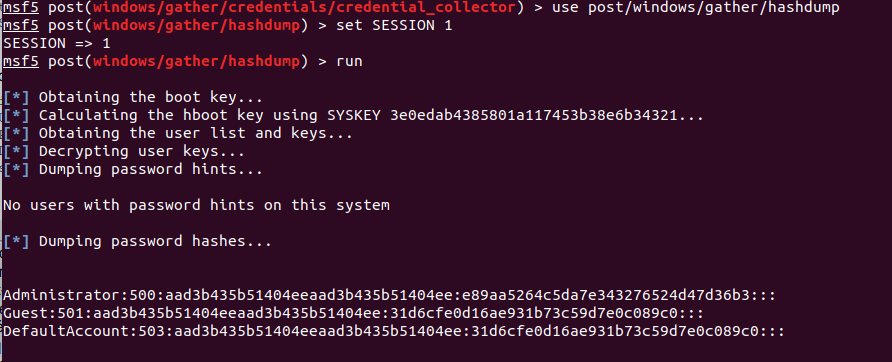
\includegraphics[width=17cm, height=7cm]{hashdump_SAM_3_3.PNG}
	\caption*{Résultat du hashdump montrant le contenu de la SAM}
\end{figure}

\begin{figure}[!h]
	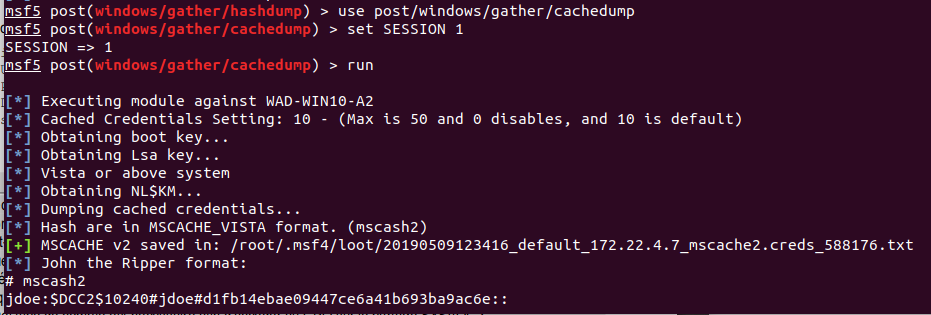
\includegraphics[width=17cm, height=7cm]{mscash_3_3.PNG}
	\caption*{Contenu du MS-CACHE}
\end{figure}

\begin{figure}[!h]
	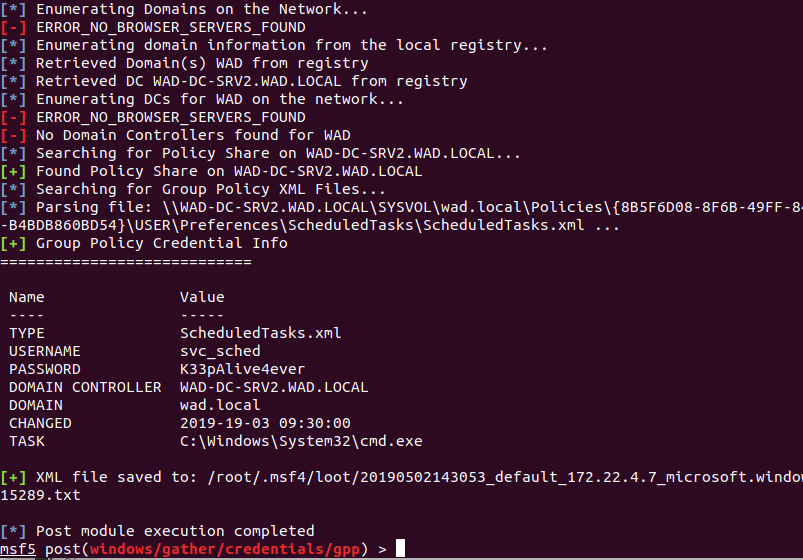
\includegraphics[width=17cm, height=7cm]{3_3_first_gather_gpp.PNG}
	\caption*{Résultat du GPP}
\end{figure}

\newpage

\section*{Kerberoast}

\subsection*{Réponses aux questions}
\par P18 : get\_user\_spns renvoie une seule entrée, car un seul arbitrary spn (MSSQL) , avec un mot de passe plus court et quasiment jamais changé
\par P19 : MSSQLSvc/WAD-SQLSRV01.WAD.local:1433
\par P20 : adm-sql avec le mot de passe Andromeda1
\par P21	: 

\subsection*{Résultat des Manipulations}

\newpage

\section*{Mouvements latéraux}

\subsection*{Réponses aux questions}
\par P22	:
\par P23	: Il  faut des privilèges administrateurs car psexec lance des services Windows et il faut être admin pour le faire
\par P24	: [dire que module a été utilie pour trouver le ntlm etc]
\par P25	: 
\par P26	: Pour des configurations larges sur tout les domaines, pour promouvoir des utilisateurs en admin, etc
\par P27	: En empêchant l'accès à l'ordinateur qui contient le Domain Admin depuis le réseau par exemple

\subsection*{Résultat des Manipulations}

\newpage

\section*{Persistance}

\subsection*{Réponses aux questions}
\par P28	: On reçoit un system error comme quoi on n'est pas log avec un utilisateur ayant les bons privilèges
\par P29	: La seconde fois le système nous le permet. En forgeant le golden ticket, on a accès aux droits de tous les utilisateurs,
y compris celui du Domain Admin, ce qui nous donne le droit de faire ce qu'on veut sur cette machine, y compris monter un partage.
\par P30	: 
\par P31	: Il peut être valide pendant plusieurs années
\par P32	: 

\subsection*{Résultat des Manipulations}


\end{document}



